\documentclass{article}
\usepackage{physics}
\usepackage{graphicx}
\usepackage{caption}
\usepackage{amsmath}
\usepackage{bm}
\usepackage{framed}
\usepackage{authblk}
\usepackage{empheq}
\usepackage{amsfonts}
\usepackage{esint}
\usepackage[makeroom]{cancel}
\usepackage{dsfont}
\usepackage{centernot}
\usepackage{mathtools}
\usepackage{subcaption}
\usepackage{bigints}
\usepackage{amsthm}
\theoremstyle{definition}
\newtheorem{lemma}{Lemma}
\newtheorem{defn}{Definition}[section]
\newtheorem{prop}{Proposition}[section]
\newtheorem{rmk}{Remark}[section]
\newtheorem{thm}{Theorem}[section]
\newtheorem{exmp}{Example}[section]
\newtheorem{prob}{Problem}[section]
\newtheorem{sln}{Solution}[section]
\newtheorem*{prob*}{Problem}
\newtheorem{exer}{Exercise}[section]
\newtheorem*{exer*}{Exercise}
\newtheorem*{sln*}{Solution}
\usepackage{empheq}
\usepackage{tensor}
\usepackage{xcolor}
%\definecolor{colby}{rgb}{0.0, 0.0, 0.5}
\definecolor{MIT}{RGB}{163, 31, 52}
\usepackage[pdftex]{hyperref}
%\hypersetup{colorlinks,urlcolor=colby}
\hypersetup{colorlinks,linkcolor={MIT},citecolor={MIT},urlcolor={MIT}}  
\usepackage[left=1in,right=1in,top=1in,bottom=1in]{geometry}
\setcounter{MaxMatrixCols}{20}
\usepackage{newpxtext,newpxmath}
\newcommand*\widefbox[1]{\fbox{\hspace{2em}#1\hspace{2em}}}

\newcommand{\p}{\partial}
\newcommand{\R}{\mathbb{R}}
\newcommand{\C}{\mathbb{C}}
\newcommand{\lag}{\mathcal{L}}
\newcommand{\nn}{\nonumber}
\newcommand{\ham}{\mathcal{H}}
\newcommand{\M}{\mathcal{M}}
\newcommand{\I}{\mathcal{I}}
\newcommand{\K}{\mathcal{K}}
\newcommand{\F}{\mathcal{F}}
\newcommand{\w}{\omega}
\newcommand{\lam}{\lambda}
\newcommand{\al}{\alpha}
\newcommand{\be}{\beta}
\newcommand{\x}{\xi}

\newcommand{\G}{\mathcal{G}}

\newcommand{\f}[2]{\frac{#1}{#2}}

\newcommand{\ift}{\infty}

\newcommand{\lp}{\left(}
\newcommand{\rp}{\right)}

\newcommand{\lb}{\left[}
\newcommand{\rb}{\right]}

\newcommand{\lc}{\left\{}
\newcommand{\rc}{\right\}}


\newcommand{\V}{\mathbf{V}}
\newcommand{\U}{\mathcal{U}}
\newcommand{\Id}{\mathcal{I}}
\newcommand{\D}{\mathcal{D}}
\newcommand{\Z}{\mathcal{Z}}

%\setcounter{chapter}{-1}


\usepackage{enumitem}



\usepackage{listings}
\captionsetup[lstlisting]{margin=0cm,format=hang,font=small,format=plain,labelfont={bf,up},textfont={it}}
\renewcommand*{\lstlistingname}{Code \textcolor{violet}{\textsl{Mathematica}}}
\definecolor{gris245}{RGB}{245,245,245}
\definecolor{olive}{RGB}{50,140,50}
\definecolor{brun}{RGB}{175,100,80}

%\hypersetup{colorlinks,urlcolor=colby}
\lstset{
	tabsize=4,
	frame=single,
	language=mathematica,
	basicstyle=\scriptsize\ttfamily,
	keywordstyle=\color{black},
	backgroundcolor=\color{gris245},
	commentstyle=\color{gray},
	showstringspaces=false,
	emph={
		r1,
		r2,
		epsilon,epsilon_,
		Newton,Newton_
	},emphstyle={\color{olive}},
	emph={[2]
		L,
		CouleurCourbe,
		PotentielEffectif,
		IdCourbe,
		Courbe
	},emphstyle={[2]\color{blue}},
	emph={[3]r,r_,n,n_},emphstyle={[3]\color{magenta}}
}

\newcommand{\diag}{\text{diag}}
\newcommand{\psirot}{\ket{\psi_\text{rot}(t)} }
\newcommand{\RWA}{\ham_\text{rot}^\text{RWA}}

% 3j symbol
\newcommand{\tj}[6]{ \begin{pmatrix}
		#1 & #2 & #3 \\
		#4 & #5 & #6 
\end{pmatrix}}


\begin{document}
\begin{framed}
\noindent Name: \textbf{Huan Q. Bui}\\
Course: \textbf{8.421 - AMO I}\\
Problem set: \textbf{\#7}\\
Due: Friday, April 1, 2022.
\end{framed}
	
	
\noindent \textbf{1. Spherical Harmony.} We want to evaluate matrix elements
\begin{align*}
\langle J' m'_J| Y_{LM} |Jm_J\rangle = \int \,d\Omega \, Y^*_{J'm'_J} Y_{LM} Y_{Jm_J} .
\end{align*}
To do this, we consider two particles with angular momenta $\bm{j}_1$ and $\bm{j}_2$. The total angular momentum is $\bm{J} = \bm{j}_1 + \bm{j}_2$. We can go between the coupled and uncoupled basis via 
\begin{align*}
| (j_1j_2) JM\rangle &= \sum_{m_1,m_2} |j_1m_1\rangle | j_2m_2\rangle \langle j_1m_1j_2m_2 | JM\rangle\\
|j_1m_1\rangle | j_2m_2\rangle &= \sum_{J,M} |(j_1j_2)JM\rangle \langle JM| j_1m_1j_2m_2\rangle.
\end{align*}

The sum over $M$ has only one nonzero term $M=m_1+m_2$, and $|j_1-j_2| < J < j_1+j_2$. We also have the wavefunction of each particle at polar angle $\Omega_i = (\theta_1,\phi_i)$ is
\begin{align*}
\langle \Omega_i | j_i m_i \rangle = Y_{j_im_i}(\Omega_i).
\end{align*}
For the state of definite total angular momentum, we have
\begin{align*}
\Phi_{JM}(\Omega_1,\Omega_2) = \langle \Omega_1 ,\Omega_2| (j_1j_2)JM\rangle.
\end{align*}
Now consider the function 
\begin{align*}
F_{JM}(\Omega) \equiv \langle \Omega,\Omega| (j_1j_2)JM\rangle
\end{align*}
where $\Omega_1 = \Omega_2 = \Omega$. This is a wavefunction of an effective particle with angular momentum quantum numbers $J,M$. Indeed, it inherits its eigenvalues $\bm{J}^2$ and $J_z$ from $\Phi_{JM}(\Omega_1,\Omega_2)$. We conclude that $F_{JM}(\Omega)$ must be proportional to the spherical harmonic $Y_{JM}(\Omega)$. Let us call
\begin{align*}
F_{JM}(\Omega) = A_{(j_1j_2)J} Y_{JM}(\Omega). 
\end{align*}
The factor $A_{(j_1j_2)J}$ cannot depend on $M$ as $F_{JM}$ must behave exactly like $Y_{JM}$, in particular when acted upon by $J_{\pm}$ which changes $M$. From here we have that
\begin{align*}
A_{(j_1j_2)J} Y_{JM}(\Omega) = \sum_{m_1,m_2}  \langle j_1m_1j_2m_2 | JM\rangle Y_{j_1m_1}(\Omega) Y_{j_2m_2}(\Omega).
\end{align*}


\begin{enumerate}[label=(\alph*)]
	\item To find $A_{(j_1j_2)J}$ we consider the special case where $\Omega = (\theta=0,\phi)$. In this case, we have that
	\begin{align*}
	Y_{j_im_i}(\Omega) = Y_{j_im_i}(\theta=0,\phi) = \sqrt{\f{2j_i+1}{4\pi}} \delta_{m_i0}.
	\end{align*}
	From the equation above we find that
	\begin{align*}
	A_{(j_1j_2)J} \sqrt{\f{2J+1}{4\pi}} \delta_{M0} = \sum_{m_1,m_2}  \langle j_1m_1j_2m_2 | JM\rangle \sqrt{\f{2j_1+1}{4\pi}} \delta_{m_10} \sqrt{\f{2j_2+1}{4\pi}} \delta_{m_20}.
	\end{align*}
	This equation is nontrivial if $M=m_1=m_2 = 0$, in which case we can solve for $A_{(j_1j_2)J}$:
	\begin{align*}
	\boxed{A_{(j_1,j_2)J} =   \sqrt{\f{(2j_1+1)(2j_2+1)}{4\pi(2J+1)}} \langle j_1 0 j_2 0 | J 0  \rangle }
	\end{align*}
	
	
	\item By applying $\langle \Omega,\Omega|$ to the LHS of 
	\begin{align*}
	|j_1m_1\rangle | j_2m_2\rangle = \sum_{J,M} |(j_1j_2)JM\rangle \langle JM| j_1m_1j_2m_2\rangle
	\end{align*}
	we find that
	\begin{align*}
	\boxed{Y_{j_1m_1} (\Omega) Y_{j_2m_2} (\Omega) }
	&= \sum_{J,M} F_{JM}(\Omega) \langle JM| j_1m_1j_2m_2\rangle \\
	&= \sum_{J,M} A_{(j_1j_2)J} Y_{JM}(\Omega) \langle JM| j_1m_1j_2m_2\rangle\\
	&= \boxed{\sum_{J,M} \sqrt{\f{(2j_1+1)(2j_2+1)}{4\pi(2J+1)}} \langle j_1 0 j_2 0 | J 0  \rangle  \langle JM| j_1m_1j_2m_2\rangle Y_{JM}(\Omega)}
	\end{align*}
	
	\item It remains to find the matrix element given at the top. To do this, we simply plug things in and use orthonormality of spherical harmonics:
	\begin{align*}
	\boxed{\langle j_3 m_3| Y_{j_2m_2} |j_1m_1\rangle }
	&= \int \,d\Omega \, Y^*_{j_3m_3}(\Omega) Y_{j_2m_2}(\Omega) Y_{j_1m_1}(\Omega) \\
	&= \int \,d\Omega \, Y^*_{j_3m_3}(\Omega) \textcolor{blue}{\sum_{J,M} \sqrt{\f{(2j_1+1)(2j_2+1)}{4\pi(2j_3+1)}} \langle j_1 0 j_2 0 | j_3 0  \rangle  \langle j_3 m_3| j_1 m_1 j_2m_2\rangle Y_{JM}(\Omega)}\\
	&= \sqrt{\f{(2j_1+1)(2j_2+1)}{4\pi(2j_3+1)}} \langle j_1 0 j_2 0 | j_3 0  \rangle  \langle j_3 m_3| j_1 m_1 j_2m_2\rangle \underbrace{\int \, d\Omega Y^*_{j_3m_3}(\Omega) Y_{j_3m_3}(\Omega) }_{1}\\
	&= \boxed{ \sqrt{\f{(2j_1+1)(2j_2+1)}{4\pi(2j_3+1)}} \langle j_1 0 j_2 0 | j_3 0  \rangle  \langle j_3 m_3| j_1 m_1 j_2m_2\rangle}
	\end{align*}
	
	
\end{enumerate}


\noindent \textbf{2. Dipole Operator.} A symmetric top molecule has a Hamiltonian $\ham = B\bm{J}^2$, with $B$ the rotational constant. The dipole moment operator is $\hat{\bm{d}} = d \hat{\bm{r}}$, with $d$ the value of the ``permanent dipole moment'' (in the molecular frame). 

\begin{enumerate}[label=(\alph*)]
	\item We will prove the spherical tensor decomposition:
	\begin{align*}
	\sum_m C_{1m}^* \hat{\bm{e}}_m = \sum_m C_{1m} \hat{\bm{e}}_m = \hat{\bm{r}}
	\end{align*}
	where $C_{1m}(\theta,\phi) = \sqrt{4\pi/3} Y_{1m}(\theta,\phi)$,
	\begin{align*}
	\hat{\bm{e}}_\pm = \mp \f{\hat{\bm{e}}_x \pm i \hat{\bm{e}}_y}{\sqrt{2}} \quad\quad \hat{\bm{e}}_0 = \hat{\bm{e}}_z
	\end{align*}
	To this end, we simply write everything out explicitly. We will show that the left-most term is equal to $\hat{\bm{r}}$. Once done, the other equality follows immediately from the fact that $\hat{\bm{r}}$ is real (and therefore the second term is equal to the (conjugate of) the first term). 
	\begin{align*}
	&C_{1-}^* \hat{\bm{e}}_{-} + 
	C_{10}^* \hat{\bm{e}}_{0}  + 
	C_{1+}^* \hat{\bm{e}}_{+}\\
	=\,\, &\f{1}{2}e^{+i\phi} \sqrt{\f{3}{2\pi}} \sqrt{\f{4\pi}{3}} \sin\theta  \f{\hat{\bm{e}}_x - i \hat{\bm{e}}_y}{\sqrt{2}} 
	+ \f{1}{2}\sqrt{\f{3}{\pi}} \sqrt{\f{4\pi}{3}} \cos\theta  \hat{\bm{e}}_z 
	+ \f{1}{2}e^{-i\phi} \sqrt{\f{3}{2\pi}} \sqrt{\f{4\pi}{3}} \sin\theta  \f{\hat{\bm{e}}_x + i \hat{\bm{e}}_y}{\sqrt{2}} \\
	=\,\, & \sin\theta\cos\phi\, {\hat{\bm{e}}}_x + \sin\theta\sin\phi\, {\hat{\bm{e}}}_y + \cos\theta \,{\hat{\bm{e}}}_z\\
	=\,\, & \hat{\bm{r}}. \quad\quad\quad \checkmark
	\end{align*}
	
	
	\item Now we will show that 
	\begin{align*}
	\hat{\bm{e}}_m^* \cdot \hat{\bm{e}}_n = \sum_p \delta_{mp}\delta_{np} = \delta_{mn}.
	\end{align*}
	It suffices to demonstrate the following cases:
	\begin{align*}
	\hat{\bm{e}}_+^*\cdot \hat{\bm{e}}_- = - \f{\hat{\bm{e}}_x - i \hat{\bm{e}}_y}{\sqrt{2}} \cdot  \f{\hat{\bm{e}}_x - i \hat{\bm{e}}_y}{\sqrt{2}} = 0  \iff \hat{\bm{e}}_-^*\cdot \hat{\bm{e}}_+ = 0
	\end{align*}
	and
	\begin{align*}
	\hat{\bm{e}}_\pm^*\cdot \hat{\bm{e}}_\pm =   \f{\hat{\bm{e}}_x \mp i \hat{\bm{e}}_y}{\sqrt{2}} \cdot  \f{\hat{\bm{e}}_x \mp i \hat{\bm{e}}_y}{\sqrt{2}} = \f{2}{2} = 1. 
	\end{align*}
	With these we are done. 
	
	
	\item Suppose we have two unit vectors $\hat{\bm{r}}$ and $\hat{\bm{r}}'$ pointing in the direction of solid angle $(\theta,\phi)$ and $(\theta',\phi')$. Let us call $\Theta$ the angle between the vectors, then we have
	\begin{align*}
	\cos\Theta &= \hat{\bm{r}} \cdot \hat{\bm{r}}' \\
	&= \sum_{m,n} C_{1m}(\theta,\phi)C_{1n}^*(\theta',\phi')\, \hat{\bm{e}}_m^* \cdot  \hat{\bm{e}}_{n}\\
	&= \sum_{m,n} C_{1m}(\theta,\phi)C_{1n}^*(\theta',\phi')\delta_{mn}\\
	&= \sum_m C_{1m}(\theta,\phi)C_{1m}^*(\theta',\phi')\\
	&= \cos\theta \cos\theta' + \f{1}{2}e^{-i\phi-i\phi'}\sin\theta\sin\theta'+\f{1}{2}e^{i\phi + i\phi'}\sin\theta\sin\theta' \\
	&= \cos\theta\cos\theta' + \cos(\phi - \phi')\sin\theta\sin\theta',
	\end{align*}
	as expected from standard geometry. A generalization of this result (for which $l=1$) is 
	\begin{align*}
	\textcolor{black}{P_l(\cos\Theta) = \sum_m C_{lm}^*(\theta,\phi) C_{lm}(\theta',\phi') }
	\end{align*}
	where 
	\begin{align*}
	C_{lm}(\theta,\phi) = \sqrt{\f{4\pi}{2l+1}}Y_{lm}(\theta,\phi).
	\end{align*}
	The proof is done by setting one of the unit vectors the $z$-axis, and the angles simplify.
	
	\item The electric field can be written 
	\begin{align*}
	\bm{E} 
	&= E_z \hat{\bm{e}}_z + E_x \hat{\bm{e}}_x + E_y \hat{\bm{e}}_y\\
	&= E_0 \hat{\bm{e}}_0 + E_+ \hat{\bm{e}}_+ + E_- \hat{\bm{e}}_-\\
	&= \sum_m E_m^* \hat{\bm{e}}_m = \sum_m E_m \hat{\bm{e}}_m^* 
 	\end{align*}
 	where $E_0, E_\pm$ defined in terms of $E_{x,y,z}$ in a similar way as the $\hat{\bm{e}}_{m}$'s are defined in terms of $\hat{\bm{e}}_{x,y,z}$. The dipole operator may be decomposed into spherical harmonics as 
 	\begin{align*}
 	-\hat{\bm{d}} \cdot \bm{E} &= -d \hat{\bm{r}} \cdot \mathbf{E} \\
 	&= -d \sum_{m,n} C_{1m}^* E_n \hat{\bm{e}}_m \cdot  \hat{\bm{e}}_n^* = -d \sum_{m,n} C_{1m} E_n^* \hat{\bm{e}}_m^* \cdot  \hat{\bm{e}}_n\\
 	&= -d\sum_m C^*_{1m}E_m = -d\sum_m C_{1m}E_m^*.
 	\end{align*}
	
	\item (Extra credit) Take $\bm{E} = E\hat{\bm{e}}_z$. The matrix elements of the Hamiltonian $\ham = B \bm{J}^2 - \hat{\bm{d}} \cdot \bm{E}$ in the $\{ |J m_J\rangle  \}$ basis are given by 
	\begin{align*}
	\langle J' m_{J'} | \ham | J m_J \rangle &=  B J(J+1)\delta_{JJ'}\delta_{m_{J'}m_J} - dE \langle J' m_{J'} | C_{10} | J m_J \rangle\\
	&= B J(J+1)\delta_{JJ'}\delta_{m_{J'}m_J} - dE \sqrt{\f{4\pi}{3}} \underbrace{\int \,d\Omega \, Y_{J' m_{J'}}^* Y_{10} Y_{J m_J}} \\
	&= B J(J+1)\delta_{JJ'}\delta_{m_{J'}m_J} -dE  \sqrt{\f{(2J+1)(2+1)}{3(2J'+1)}} \langle (J, 0) (1,0) | (J', 0)  \rangle  \langle J' m_{J'}|(J m_J)(1,0)\rangle\\
	&= B J(J+1)\delta_{JJ'}\delta_{m_{J'}m_J} -dE  \sqrt{\f{(2J+1)(2+1)}{3(2J'+1)}} \langle (J, 0) (1,0) | (J', 0)  \rangle  \langle J' m_{J'}|(J m_J)(1,0)\rangle.
	\end{align*}
	where we have used the fact that $C_{10} = C_{10}^*$ and remove the conjugation symbol. To get the matrix elements in the second term, we must use Wigner's 3-j symbols:
	\begin{align*}
	\langle j_1 m_1 j_2 m_2 | J M \rangle = (-1)^{-j_1 +j_2 -M} \sqrt{2J+1} 
	\tj{j_1}{j_2}{J}{m_1}{m_2}{-M}
	\end{align*}
	which with we write the Hamiltonian matrix elements as 
	\begin{align*}
	\langle J' m_{J'} | \ham | J m_J \rangle = &\,\,B J(J+1)\delta_{JJ'}\delta_{m_{J'}m_J} 
	\\
	&-dE \sqrt{\f{(2J+1)(2+1)}{3(2J'+1)}} 
	(-1)^{-J + 1} (-1)^{-J + 1 -m_{J'}} \sqrt{2J'+1} \sqrt{2J'+1} \tj{J}{1}{J'}{0}{0}{0} 
	 \tj{J}{1}{J'}{m_J}{0}{-m_{J'}} \\
	= &\,\, B J(J+1)\delta_{JJ'}\delta_{m_{J'}m_J}  -dE (-1)^{-m_{J'}} \sqrt{\f{(2J+1)(2+1)(2J'+1)}{3}} \tj{J}{1}{J'}{0}{0}{0} 
	\tj{J}{1}{J'}{m_J}{0}{-m_{J'}}.
	\end{align*}
	Using MATLAB, we can generate this matrix and diagonalize to find the eigenstates and their energies. Since it is convenient, I actually generated the Hamiltonian and carried out exact diagonalization in MATLAB but then plotted the probabilities in using \texttt{SphericalPlot3D[]} in Mathematica. Perhaps the grader will tell me that this solution is \textit{cursed}. Figure \ref{fig:energies} shows the first six energy levels up to an electric field $E \approx 10B/d$. For this calculation, I have picked $J_\text{max} = 10$.\\
	
	
	Using Mathematica, we plot $\abs{\bra{\theta,\phi}\ket{\Psi}}^2$ of the lowest state for $dE/B = 0, 1, 10$. To do this, I have used MATLAB to find the lowest energy eigenstate for each value of $dE/B$. Then, I express these states in terms of spherical harmonics by identifying each entry of the state vector with the correct $\ket{Jm_J}$ state in the basis. For this part of the problem, I have used $J_\text{max}=4$.  See Figures \ref{fig:0}, \ref{fig:1}, \ref{fig:10} for the results.	
	
	
	
	\begin{figure}[!htb]
		\centering
		\includegraphics[width=0.8\textwidth]{energies.eps}
		\caption{Energies of the first six energy levels p to an electric field $E \approx 10 B/d$.}
		\label{fig:energies}
	\end{figure}


	\begin{figure}[!htb]
		\centering
		\begin{subfigure}{.5\textwidth}
			\centering
			\includegraphics[width=0.9\linewidth]{e0.eps}
			\caption{$\abs{\bra{\theta,\phi}\ket{\Psi}}^2$ for $dE/B=0$.}
			\label{fig:0}
		\end{subfigure}%
		\begin{subfigure}{.5\textwidth}
			\centering
			\includegraphics[width=.9\linewidth]{e1.eps}
			\caption{$\abs{\bra{\theta,\phi}\ket{\Psi}}^2$ for $dE/B=1$.}
			\label{fig:1}
		\end{subfigure}
	\end{figure}

	\begin{figure}[!htb]
		\centering
		\includegraphics[width=0.5\textwidth]{e10.eps}
		\caption{$\abs{\bra{\theta,\phi}\ket{\Psi}}^2$ for $dE/B=10$.}
		\label{fig:10}
	\end{figure}
	
	
	MATLAB code for calculating:
	\begin{lstlisting}
	clear all
	close all
	
	J = 10;
	strength = 0:0.05:10;
	size = (J+1)^2;
	H = zeros(size,size);
	
	% creat a basis for the Hamiltonian
	basis = [];
	
	for j = 0:1:J
	for mj = -j:1:j
	basis = [basis; [j mj]];
	end
	end
	
	%%%%%%%%%%%%%%%%%%%%%%%%%%%%%%%%%%%%%%%%%%%%%%%%%%%%%%%%
	%%%%%%%%%%%%%%%%%%%%%%%%%%%%%%%%%%%%%%%%%%%%%%%%%%%%%%%%
	
	%%% first plot energies as a fn of dE/B
	
	stark = figure(1);
	for a = strength % loop over field strengths
	% create the Hamiltonian, element-by-element
	for r = 1:size
	j = basis(r,1);
	mj = basis(r,2);
	for c = 1:size     
	jj = basis(c,1);  
	mjj = basis(c,2);
	
	H(r,c) = j*(j+1)*(j==jj)*(mj==mjj)...
	-a*(-1)^(-mjj)*sqrt((2*j+1)*(2*1+1)*(2*jj+1)/3)...
	*Wigner3j([j,1,jj],[0,0,0])*Wigner3j([j,1,jj],[mj,0,-mjj]);             
	end
	end
	% diag n plot eigenvalues associated with field strength a = dE/B
	energies = eig(H);
	hold on 
	plot(a*ones(size), energies, '.', 'Color', 'red', 'MarkerSize',4);
	end
	
	% disp(H)
	
	% plot includes up to 6 lowest energies only
	
	hold off
	%title('Energy vs dE/B')
	ylim([-6.5 10])
	xlabel('dE/B')
	ylabel('Energy/B')
	
	
	%%%%%%%%%%%%%%%%%%%%%%%%%%%%%%%%%%%%%%%%%%%%%%%%%%%%%%%%
	%%%%%%%%%%%%%%%%%%%%%%%%%%%%%%%%%%%%%%%%%%%%%%%%%%%%%%%%
	%%%%%%%%%%%%%%%%%%%%%%%%%%%%%%%%%%%%%%%%%%%%%%%%%%%%%%%%
	%%%%%%%%%%%%%%%%%%%%%%%%%%%%%%%%%%%%%%%%%%%%%%%%%%%%%%%%
	
	
	% now find the lowest state and associated energy for various a = dE/B
	% then take result over to mathematica to plot wavefunction^2
	
	strength = [0 1 10];
	wavefunction = 0;
	
	for a = strength % loop over field strengths
	% create the Hamiltonian, element-by-element
	for r = 1:size
	j = basis(r,1);
	mj = basis(r,2);
	for c = 1:size     
	jj = basis(c,1);  
	mjj = basis(c,2);
	
	H(r,c) = j*(j+1)*(j==jj)*(mj==mjj)...
	-a*(-1)^(-mjj)*sqrt((2*j+1)*(2*1+1)*(2*jj+1)/3)...
	*Wigner3j([j,1,jj],[0,0,0])*Wigner3j([j,1,jj],[mj,0,-mjj]);             
	end
	end
	% diag n plot eigenvalues associated with field strength a = dE/B
	[state,energy] = eigs(H,1,'SA');
	disp('Ground state energy:')
	disp(energy)
	disp('Ground state:')
	disp(state) 
	
	end
	
	\end{lstlisting}
	
	
	Mathematica code for plotting:
	\begin{lstlisting}
	(*dE/B=0 ---> |0,0> state*)
	
	Energy1 = 0;
	
	State1 = SphericalHarmonicY[0, 0, \[Theta], \[Phi]];
	
	SphericalPlot3D[
	Conjugate[State1]*State1, {\[Theta], 0, Pi}, {\[Phi], 0, 2 Pi}, 
	PlotRange -> All]
	
	
	(*dE/B=1 ---> get superposition state*)
	
	Jmax2 = 4;
	
	Base2 = Flatten[
	Table[SphericalHarmonicY[J, mJ, \[Theta], \[Phi]], {J, 0, 
	Jmax2}, {mJ, -J, J}], 1];
	
	Energy2 = -0.1577;
	
	State2 = {-0.9644, 0.0000, -0.2634, -0.0000, -0.0000,
	0.0000, -0.0222, -0.0000, -0.0000, 0.0000, 0.0000, 
	0.0000, -0.0009, -0.0000, 0.0000, 0.0000, 0.0000, -0.0000, -0.0000,
	0.0000, -0.0000, -0.0000, 0.0000, -0.0000, 0.0000};
	
	State2 = State2/Norm[State2];
	
	wfn2 = Dot[Base2, State2]
	
	-0.27206 - 0.128702 Cos[\[Theta]] - 
	0.0070019 (-1 + 3 Cos[\[Theta]]^2) - 
	0.000335869 (-3 Cos[\[Theta]] + 5 Cos[\[Theta]]^3)
	
	SphericalPlot3D[
	Conjugate[wfn2]*wfn2, {\[Theta], 0, Pi}, {\[Phi], 0, 2 Pi}, 
	AspectRatio -> Full]
	
	
	(*dE/B=10 ---> get superposition state*)
	
	Jmax3 = 4;
	
	Base3 = Flatten[
	Table[SphericalHarmonicY[J, mJ, \[Theta], \[Phi]], {J, 0, 
	Jmax2}, {mJ, -J, J}], 1];
	
	Energy3 = -6.0448;
	
	State3 = {-0.6477, 0.0000, -0.6782, -0.0000, 
	0.0000, -0.0000, -0.3323, -0.0000, 0.0000, -0.0000, 0.0000, 
	0.0000, -0.0987, -0.0000, -0.0000, 0.0000, 0.0000, 0.0000, -0.0000,
	0.0000, -0.0191, -0.0000, 0.0000, -0.0000, 0.0000};
	
	State3 = State3/Norm[State3];
	
	wfn3 = Dot[Base3, State3]
	
	-0.182713 - 0.33137 Cos[\[Theta]] - 
	0.104805 (-1 + 3 Cos[\[Theta]]^2) - 
	0.0368325 (-3 Cos[\[Theta]] + 5 Cos[\[Theta]]^3) - 
	0.0020205 (3 - 30 Cos[\[Theta]]^2 + 35 Cos[\[Theta]]^4)
	
	SphericalPlot3D[
	Conjugate[wfn3]*wfn3, {\[Theta], 0, Pi}, {\[Phi], 0, 2 Pi}, 
	PlotRange -> All, AspectRatio -> Full]
	
	
	\end{lstlisting}

	
\end{enumerate}

\noindent \textbf{3. The Stark Effect in Hydrogen.}

\begin{enumerate}[label=(\alph*)]
	\item \textbf{Stark quenching of the $2S$ state.} In hydrogen, the $2S$ state is metastable. In the absence of external electric fields, its lifetime is $1/8$ seconds. When an external electric field is applied, the $2S$ becomes mixed with the $2P$ state, which is strongly coupled to the ground state. The $2P$ state lifetime is only 1.6 ns. Depending on the strength of the electric field, the lifetime of the $2S$ state can be shortened by many orders og magnitude. This process is known as ``quenching.'' To see how this works, we will look at how the amplitude $a(t)$ of $\ket{a} $ ($2S$ state) evolves ocer time in the presenece of a DC Stark perturbation with matrix element $\hbar V  =\bra{b} e\bm{E}\cdot \bm{r} \ket{a}$ where $\ket{b}$ stands for the $2P$ state.\\
	
	
	Assuming that the atom is initially in the $2S$ state, i.e., $a(0) = 1, b(0) = 0$. Working in the interaction picture, we can derive the following differential equations for $a(t)$ and $b(t)$: 
	\begin{align*}
	i\dot a &= V^* e^{i\omega_0 t} b - i \f{\Gamma_a}{2}a\\
	i\dot b &= V e^{-i\omega_0 t} a - i \f{\Gamma_b}{2}b
	\end{align*}
	where $\Gamma_a = 8$ s$^{-1}$ and $\Gamma_b = 6.3 \times 10^8$ s$^{-1}$. Here, $\hbar \omega_0$ is the energy difference $E_a - E_b$. To solve these equations, we make the following ansatz
	\begin{align*}
	a(t) &= a_1 e^{-\mu_1 t} + a_2 e^{-\mu_2 t}\\
	b(t) &= b_1 e^{-(\mu_1 + i\omega_0)t} + b_2 e^{-(\mu_2 + i\omega_0)t}
	\end{align*}
	where $a_1,a_2,b_1,b_2$ are constants. Applying the initial condition $a(0) = 1, b(0) = 0$ we find that
	\begin{align*}
	a_1 + a_2 = 1 \quad\quad \quad b_1 + b_2 =0.
	\end{align*}
	With this, we may write our ansatz as 
	\begin{align*}
	a(t) &= a_1 e^{-\mu_1 t} + (1-a_1) e^{-\mu_2 t}\\
	b(t) &= b_1 e^{-(\mu_1 + i\omega_0)t} -b_1 e^{-(\mu_2 + i\omega_0)t}
	\end{align*}
	From this point, we may proceed using Mathematica. Plugging this ansatz into the system of differential equations above and set $t=0$, we can solve for $\mu_1$ and $\mu_2$ in terms of $a_1,b_1$. The result is 
	\begin{align*}
	{\mu_1 = \f{\Gamma_a}{2} - \f{i(a_1-1)V}{b_1} \quad\quad \mu_2 = \f{\Gamma_a}{2} - \f{ia_1V}{b_1}}
	\end{align*}
	
	It remains to find $a_1,b_1$. To this end, we pick $t=1/V$. By writing $\mu_1,\mu_2$ in terms of $a_1,b_1$, we can solve for $a_1,b_1$. The result is 
	\begin{align*}
	a_1 &= \f{1}{2} + \frac{ i (\Gamma_a- \Gamma_b) - 2 \omega_0}{2 \sqrt{-(\Gamma_a-\Gamma_b-4
			V+2 i \omega_0) (\Gamma_a-\Gamma_b+4 V+2 i \omega_0)}}\\
	b_1 &= 	-\frac{2 V}{\sqrt{-(\Gamma_a-\Gamma_b-4 V+2 i \omega_0) (\Gamma_a-\Gamma_b+4 V+2 i\omega_0)}}
	\end{align*}
	Note that there is another solution $(a_1,b_1)$, but it doesn't matter all that much what we pick to compute $\mu_1,\mu_2$ since the result is the same. So we will pick the solution above. We should simplify this even more by writing the denominator as 
	\begin{align*}
	\sqrt{-(\Gamma_a-\Gamma_b-4 V+2 i \omega_0) (\Gamma_a-\Gamma_b+4 V+2 i\omega_0)}
	&= \sqrt{16V^2 - ((\Gamma_a-\Gamma_b)+2 i\omega_0)^2}\\
	&= \sqrt{16V^2 - (\Gamma_a- \Gamma_b)^2 +4 \omega_0^2  - 4i\omega_0(\Gamma_a - \Gamma_b)}.
	\end{align*}
	Now recall that for $x,y\in \mathbb{R}$, 
	\begin{align*}
	\sqrt{x+iy} = \sqrt{\f{\sqrt{x^2+y^2} + x }{2}} + i\text{sgn}(y)\sqrt{\f{\sqrt{x^2+y^2} - x}{2}}.
	\end{align*}
	Let $x = 16V^2 - (\Gamma_a- \Gamma_b)^2 +4 \omega_0^2$ and $y = -4\omega_0(\Gamma_a - \Gamma_b) > 0$, then we have
	\begin{align*}
	\sqrt{-(\Gamma_a-\Gamma_b-4 V+2 i \omega_0) (\Gamma_a-\Gamma_b+4 V+2 i\omega_0)} &= \sqrt{x+iy} \\
	&=\sqrt{\f{\sqrt{x^2+y^2} + x }{2}} + i\sqrt{\f{\sqrt{x^2+y^2} - x}{2}}.
	\end{align*}
	From here we can calculate $\mu_1,\mu_2$:
	\begin{align*}
	\mu_1 &= \f{\Gamma_a}{4} + \f{\Gamma_b}{4} + \f{i}{4}\sqrt{x+iy} - \f{i\omega_0}{2} \\
	\mu_2 &= \f{\Gamma_a}{4} + \f{\Gamma_b}{4} - \f{i}{4}\sqrt{x+iy} - \f{i\omega_0}{2} 
	\end{align*}
	From here, we can find the real and imaginary parts of $\mu_1, \mu_2$:
	\begin{align*}
	\Re(\mu_1) 
	&= \f{\Gamma_a}{4} + \f{\Gamma_b}{4} - \f{1}{4}\sqrt{\f{\sqrt{x^2+y^2} - x}{2}}\\
	\Im(\mu_1) &= \f{1}{4} \sqrt{\f{\sqrt{x^2+y^2} + x }{2}}- \f{\omega_0}{2}\\
	\Re(\mu_2) &= \f{\Gamma_a}{4} + \f{\Gamma_b}{4}  + \f{1}{4}\sqrt{\f{\sqrt{x^2+y^2} - x}{2}}\\
	\Im(\mu_2) &=  -\f{1}{4} \sqrt{\f{\sqrt{x^2+y^2} + x }{2}}- \f{\omega_0}{2}
	\end{align*}
	
	Here, the real parts of $\mu_1,\mu_2$ give the decay rate of the $2S$ state, and the imaginary parts tell us the level shifts. With these expressions (for $\mu_1,\mu_2,a_1,a_2,b_1,b_2$) in terms of the known constants, we can write down the full solution for $a(t)$. While it is possible, I won't do that here since this is  simply plugging things into the ansatz. \\
	
	
	In the small $V$ limit, we may Taylor expand these expressions about $V = 0$ to second order in $V$ to find 
	\begin{align*}
	\Re(\mu_1) 
	&\approx \f{\Gamma_a}{4} + \f{\Gamma_b}{4} + \f{\Gamma_a}{4} - \f{\Gamma_b}{4} - \f{2(\Gamma_b-\Gamma_a)}{(\Gamma_b-\Gamma_a)^2+4\omega_0^2}V^2\\
	\Im(\mu_1) &\approx  \f{\omega_0}{2} + \f{4\omega_0}{(\Gamma_b - \Gamma_a)^2+4\omega_0^2}V^2  - \f{\omega_0}{2} = \f{4\omega_0}{(\Gamma_b - \Gamma_a)^2+4\omega_0^2} V^2 \\
	\Re(\mu_2) &\approx \f{\Gamma_a}{4} + \f{\Gamma_b}{4} - \f{\Gamma_a}{4} + \f{\Gamma_b}{4} + \f{2(\Gamma_b-\Gamma_a)}{(\Gamma_b-\Gamma_a)^2+4\omega_0^2}V^2\\
	\Im(\mu_2) &\approx  -\f{\omega_0}{2} - \f{4\omega_0}{(\Gamma_b - \Gamma_a)^2+4\omega_0^2}V^2  - \f{\omega_0}{2} = -\omega_0 + \f{4\omega_0}{(\Gamma_b - \Gamma_a)^2+4\omega_0^2} V^2.
	\end{align*}
	
	Now let us make various assumptions to simplify things. Let us assume that $\Gamma_a \ll \Gamma_b$ and $\Gamma_a \ll \mu_1, \mu_2$. From these, we have
	\begin{align*}
	\Re(\mu_1) 
	&\approx  -  \f{  \Gamma_b/2}{(\Gamma_b/2)^2+\omega_0^2} V^2\\
	\Im(\mu_1) &\approx  \f{\omega_0}{(\Gamma_b/2 )^2+\omega_0^2} V^2  \\
	\Re(\mu_2) &\approx \f{\Gamma_b}{2} +\f{  (\Gamma_b/2)}{(\Gamma_b/2)^2+\omega_0^2} V^2 \\
	\Im(\mu_2) &\approx   -\omega_0 + \f{\omega_0}{(\Gamma_b/2 )^2+\omega_0^2} V^2  
	\end{align*}
	
	
	
	
	
	
	
	
	On the other hand, we have in the large $V$ limit, $x \to 16V^2$ and $x \gg y$, and so 
	\begin{align*}
	\Re(\mu_1) &\approx \f{\Gamma_a}{4} + \f{\Gamma_b}{4} \approx \f{\Gamma_b}{4}\\
	\Im(\mu_1) &\approx  V - \f{\omega_0}{2}\\
	\Re(\mu_2) &\approx \f{\Gamma_a}{4} + \f{\Gamma_b}{4} \approx \f{\Gamma_b}{4}\\
	\Im(\mu_2) &\approx  -V - \f{\omega_0}{2}
	\end{align*}
	
	
	We see that these results agree well with perturbation theory results for Stark shift energies. 
	
	
	
	
	\item \textbf{Effect of the Lamb shift on quenching.}  Here we want to find the electric field in V/cm for which the $2S$ state lifetime is equal to 1 $\mu$s for two cases: 
	\begin{itemize}
		\item \textbf{Case 1:} Weak coupling limit $(V^2\ll \omega_0^2)$ assuming that $\omega_0$ is much smaler than the actual $2P$ linewidth $\Gamma_b$, so $\omega_0 \ll \Gamma_b$. First, we can identify from the solution above that the decay rate of the $2S$ state in the weak field limit is given by 
		\begin{align*}
		\gamma_{2S} = 2\times \f{  \Gamma_b/2}{(\Gamma_b/2)^2+\omega_0^2} V^2 \to \f{4V^2}{\Gamma_b}
		\end{align*}
		where the factor of $2$ comes from the fact that $\abs{a(t)}^2$ and $\abs{b(t)}^2$ are the relevant quantities for population. The lifetime is therefore
		\begin{align*}
		\tau_{2S} = \f{\Gamma_b}{4V^2}.
		\end{align*}
		Since $V = 3 e a_0 \mathcal{E}/\hbar$, we can set $\tau_{2S}$ to 1 $\mu$s to find that, the desired electric field strength is 
		\begin{align*}
		\mathcal{E} = \sqrt{\f{\Gamma_b}{4 (1\,\mu \text{s})(3ea_0/\hbar)^2 }} \approx \boxed{0.5203 \text{ V/cm}}
		\end{align*}
	
		
		
		\item \textbf{Case 2:} Weak field limit as above but with $\omega_0  = \omega_\text{Lamb} = 2\pi \times 1057.864 $ MHz. In this case, we find that
		\begin{align*}
		\tau_{2S} = \f{(\Gamma_b/2)^2 + \omega_0^2}{\Gamma_b V^2} \implies \mathcal{E} = \sqrt{ \f{(\Gamma_b/2)^2 + \omega_0^2}{\Gamma_b (1 \, \mu\text{s}) (3a_0 e /\hbar)^2}   } \approx \boxed{1.82 \text{ V/cm}} 
		\end{align*}
	\end{itemize}	
	Including the Lamb shift increases the electric field required by a factor of $\sim$3.5 on this time scale. \\
	
	
	$\,$\\
	
	Mathemetica code:
	\begin{lstlisting}
	(*Problem 3: Stark stuff*)
	
	In[1]:= a[t_] := a1*Exp[-m1*t] + (1 - a1)*Exp[-m2*t];
	
	In[2]:= b[t_] := b1*Exp[-(m1 + I*w0)*t] - b1*Exp[-(m2 + I*w0)*t];
	
	In[3]:= FullSimplify[
	I*a'[t] == V*Exp[I*w0*t]*b[t] - I*Ga/2*a[t]] /. {t -> 0}
	
	Out[3]= I (a1 (Ga - 2 m1) + 2 I b1 V) - 
	I ((-1 + a1) (Ga - 2 m2) + 2 I b1 V) == 0
	
	In[4]:= FullSimplify[
	I*b'[t] == V*Exp[-I*w0*t]*a[t] - I*Gb/2*b[t]] /. {t -> 0}
	
	Out[4]= I b1 (Gb - 2 m1) + 2 (-1 + a1) V - 2 a1 V - 
	I b1 (Gb - 2 (m2 + I w0)) + 2 b1 w0 == 0
	
	
	(*Solve for m1, m2*)
	
	In[5]:= Solve[{I (a1 (Ga - 2 m1) + 2 I b1 V) - 
	I ((-1 + a1) (Ga - 2 m2) + 2 I b1 V) == 0, 
	I b1 (Gb - 2 m1) + 2 (-1 + a1) V - 2 a1 V - 
	I b1 (Gb - 2 (m2 + I w0)) + 2 b1 w0 == 0}, {m1, 
	m2}] // FullSimplify
	
	Out[5]= {{m1 -> Ga/2 - (I (-1 + a1) V)/b1, m2 -> Ga/2 - (I a1 V)/b1}}
	
	
	(*Pick t=1/V, solve for a1, b1*)
	
	In[6]:= eqn1 = 
	I*a'[t] == V*Exp[I*w0*t]*b[t] - I*Ga/2*a[t] /. {t -> 1/V, 
	m1 -> Ga/2 - (I (-1 + a1) V)/b1, m2 -> Ga/2 - (I a1 V)/b1} // 
	FullSimplify
	
	Out[6]= (((-1 + a1) a1 + b1^2) E^((I (-1 + a1))/b1 - Ga/(
	2 V)) (-1 + E^(I/b1)) V)/b1 == 0
	
	In[8]:= eqn2 = 
	I*b'[t] == V*Exp[-I*w0*t]*a[t] - I*Gb/2*b[t] /. {t -> 1/V, 
	m1 -> Ga/2 - (I (-1 + a1) V)/b1, m2 -> Ga/2 - (I a1 V)/b1} // 
	FullSimplify
	
	Out[8]= E^((I (-1 + a1))/b1 - (Ga + 2 I w0)/(
	2 V)) (-1 + E^(I/b1)) (2 (-1 + 2 a1) V + 
	I b1 (Ga - Gb + 2 I w0)) == 0
	
	(*Solve for a1, b1*)
	In[9]:= Solve[{eqn1, eqn2}, {a1, b1}] // FullSimplify
	

	Out[9]= {{a1 -> (
	I Ga - I Gb + 
	Sqrt[-((Ga - Gb - 4 V + 2 I w0) (Ga - Gb + 4 V + 2 I w0))] - 
	2 w0)/(2 Sqrt[-((Ga - Gb - 4 V + 2 I w0) (Ga - Gb + 4 V + 
	2 I w0))]), 
	b1 -> -((2 V)/
	Sqrt[-((Ga - Gb - 4 V + 2 I w0) (Ga - Gb + 4 V + 
	2 I w0))])}, {a1 -> (-I Ga + I Gb + 
	Sqrt[-((Ga - Gb - 4 V + 2 I w0) (Ga - Gb + 4 V + 2 I w0))] + 
	2 w0)/(2 Sqrt[-((Ga - Gb - 4 V + 2 I w0) (Ga - Gb + 4 V + 
	2 I w0))]), 
	b1 -> (2 V)/
	Sqrt[-((Ga - Gb - 4 V + 2 I w0) (Ga - Gb + 4 V + 2 I w0))]}}
	
	In[135]:= (*Find mu1*)
	
	In[30]:= Ga/2 - (I (-1 + a1) V)/b1 // Expand
	
	Out[30]= Ga/4 + Gb/4 - 
	1/4 I Sqrt[-((Ga - Gb - 4 V + 2 I w0) (Ga - Gb + 4 V + 2 I w0))] - (
	I w0)/2
	
	In[13]:= (*Find mu2*)
	
	In[31]:= Ga/2 - (I a1 V)/b1 // Expand
	
	Out[31]= Ga/4 + Gb/4 + 
	1/4 I Sqrt[-((Ga - Gb - 4 V + 2 I w0) (Ga - Gb + 4 V + 2 I w0))] - (
	I w0)/2
	
	(*Weak field limit --> get V^2 scaling*)
	
	In[26]:= Series[
	Sqrt[(Sqrt[x^2 + y^2] - x)/2], {V, 0, 2}] // FullSimplify
	
	Out[26]= SeriesData[V, 0, {
	2^Rational[-1, 2] (
	Gab^2 - 4 w0^2 + ((Gab^2 + 4 w0^2)^2)^Rational[1, 2])^Rational[
	1, 2], 0, (-4)
	2^Rational[1, 2] ((Gab^2 + 4 w0^2)^2)^Rational[-1, 2] (
	Gab^2 - 4 w0^2 + ((Gab^2 + 4 w0^2)^2)^Rational[1, 2])^Rational[
	1, 2]}, 0, 3, 1]
	
	In[146]:= 
	Series[Sqrt[(Sqrt[x^2 + y^2] + x)/2], {V, 0, 2}] // FullSimplify
	
	Out[146]= SeriesData[V, 0, {
	2^Rational[-1, 
	2] (-Gab^2 + 4 w0^2 + ((Gab^2 + 4 w0^2)^2)^Rational[
	1, 2])^Rational[1, 2], 
	0, (4 ((Gab^2 + 4 w0^2)^2)^Rational[-1, 2]) ((-2)
	Gab^2 + 8 w0^2 + 2 ((Gab^2 + 4 w0^2)^2)^Rational[
	1, 2])^Rational[1, 2]}, 0, 3, 1]
	\end{lstlisting}




\end{enumerate}

\end{document}








